\documentclass[12pt, a4paper, oneside]{article} % Paper size, default font size and one-sided paper
%\graphicspath{{./Figures/}} % Specifies the directory where pictures are stored
%\usepackage[dcucite]{harvard}
\usepackage{tikz}
\usetikzlibrary{shapes, shadows, arrows}
\usepackage{rotating}
\usepackage{setspace}
\usepackage{pdflscape}
\usepackage[flushleft]{threeparttable}
\usepackage{multirow}
\usepackage[comma, sort&compress]{natbib}% Use the natbib reference package - read up on this to edit the reference style; if you want text (e.g. Smith et al., 2012) for the in-text references (instead of numbers), remove 'numbers' 
\usepackage{graphicx}
%\bibliographystyle{plainnat}
\bibliographystyle{agsm}
\usepackage[colorlinks = true, citecolor = blue, linkcolor = blue]{hyperref}
%\hypersetup{urlcolor=blue, colorlinks=true} % Colors hyperlinks in blue - change to black if annoying
%\renewcommand[\harvardurl]{URL: \url}
\begin{document}
\title{TikZ}
\author{Rob Hayward\footnote{University of Brighton Business School, Lewes Road, Brighton, BN2 4AT; Telephone 01273 642586.  rh49@brighton.ac.uk}} 
\date{\today}
\maketitle
\begin{abstract}
This is a file to practice the TiKz package.  Much of this comes from the minimal introduction to TiZk (in ``other'' folder). 
\end{abstract}
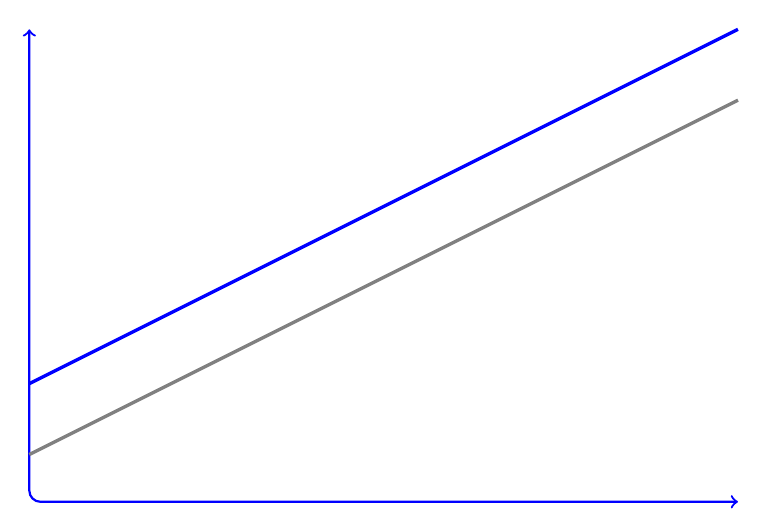
\begin{tikzpicture}[xscale = 3, yscale = 3]
%\draw[help lines] (0, 0) grid (2, 3);
\draw [<->, rounded corners, thick, blue](0, 2) -- (0, 0) -- (3, 0);
\draw [gray, very thick, domain = 0:3] plot(\x, {0.2 + \x * 0.5});
\draw [blue, very thick, domain = 0:3] plot(\x, {0.5 + \x * 0.5});
\end{tikzpicture}

\begin{figure}
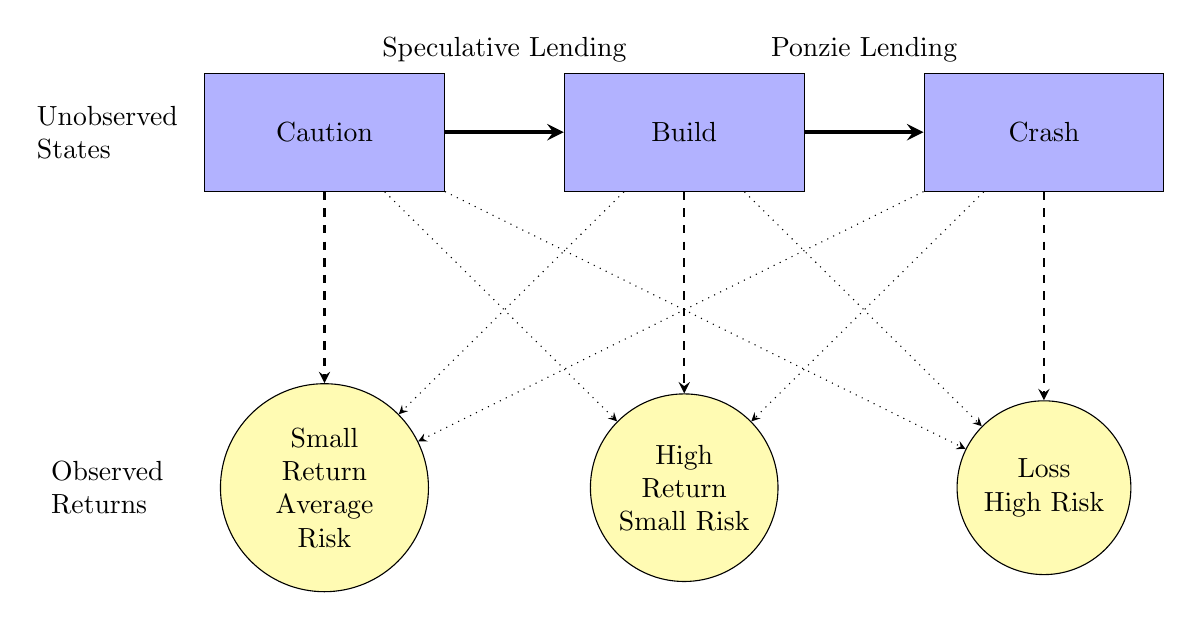
\begin{tikzpicture}
\tikzstyle{decision} = [circle, draw, fill = yellow!30, minimum height = 8mm, 
  text width = 5em, text centered];
\tikzstyle{line} = [draw, -stealth, thick]
\tikzstyle{line2} = [draw, -stealth, ultra thick]
\tikzstyle{line3} = [draw, -stealth, dashed, thick]
\tikzstyle{line4} = [draw, -stealth, dotted]
\tikzstyle{elli} = [draw, ellipse, fill = red!50, minimum height = 8mm, 
	text width = 5em, text centered]
\tikzstyle{block} = [draw, rectangle, fill = blue!30, text width = 8em, 
	text centered, minimum height = 15mm, node distance = 8em]
\node [block](Build){Build};
\node [block, left of  = Build, xshift = -5em] (Caution){Caution}; 
\node [block, right  of = Build, xshift =5em] (Crash){Crash};
\node [decision, below of = Build, yshift = -10em, align = center]
(Build2) {High Return \\ Small Risk}; 
\node [decision, below of = Crash, yshift = -10em](Crash2) {Loss \\ High Risk};
\node [decision, below of = Caution, yshift = -10em, align = center](Caution2) 
{Small \\ Return \\ Average \\ Risk};
%arrows 
\path [line3] (Caution) -- (Caution2);
\path [line3] (Build) -- (Build2);
\path [line3] (Crash) -- (Crash2);
\path [line2] (Build) -- node [yshift = 3em] {Ponzie Lending} (Crash);
\path [line2] (Caution) -- node [yshift = 3em]  {Speculative Lending} (Build);
\path [line4] (Caution) -- (Build2);
\path [line4] (Caution) -- (Crash2);
\path [line4] (Build) -- (Crash2);
\path [line4] (Build) -- (Caution2);
\path [line4] (Crash) -- (Caution2);
\path [line4] (Crash) -- (Build2);
\node [align = left, left of = Caution, xshift = -5em] {Unobserved \\ States};
\node [align = left, left of = Caution2, xshift = -5em] {Observed \\ Returns};
%\path [line] (decision1) -| node [yshift = 0.5em, 
% 	xshift = 8em] {YES} (process 1);
%\path [line3] (Crash) -- (Caution); 
% 	xshift = -8em] {NO} (process 2);
\end{tikzpicture}
%\caption{Carry Trade: Regime Change}
\end{figure}


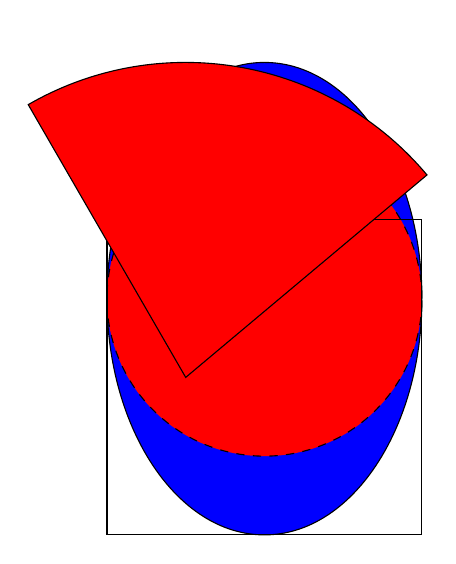
\begin{tikzpicture}
% http://www.youtube.com/watch?v=BxBJfBgntBw&list=UU7Bbc2pxojIxRglXbm_mC2g
\draw [fill = blue] (2,3) ellipse (2 and 3);
\draw [fill = red, style = dashed] (2,3) circle (2);
\draw (0, 0) rectangle (4,4);
\draw [fill = red](1,2) -- +(40:4) arc(40:120:4) -- cycle; 


\end{tikzpicture}

% Video for flow chart example
%http://www.youtube.com/watch?v=5pdQG8ZMPVA
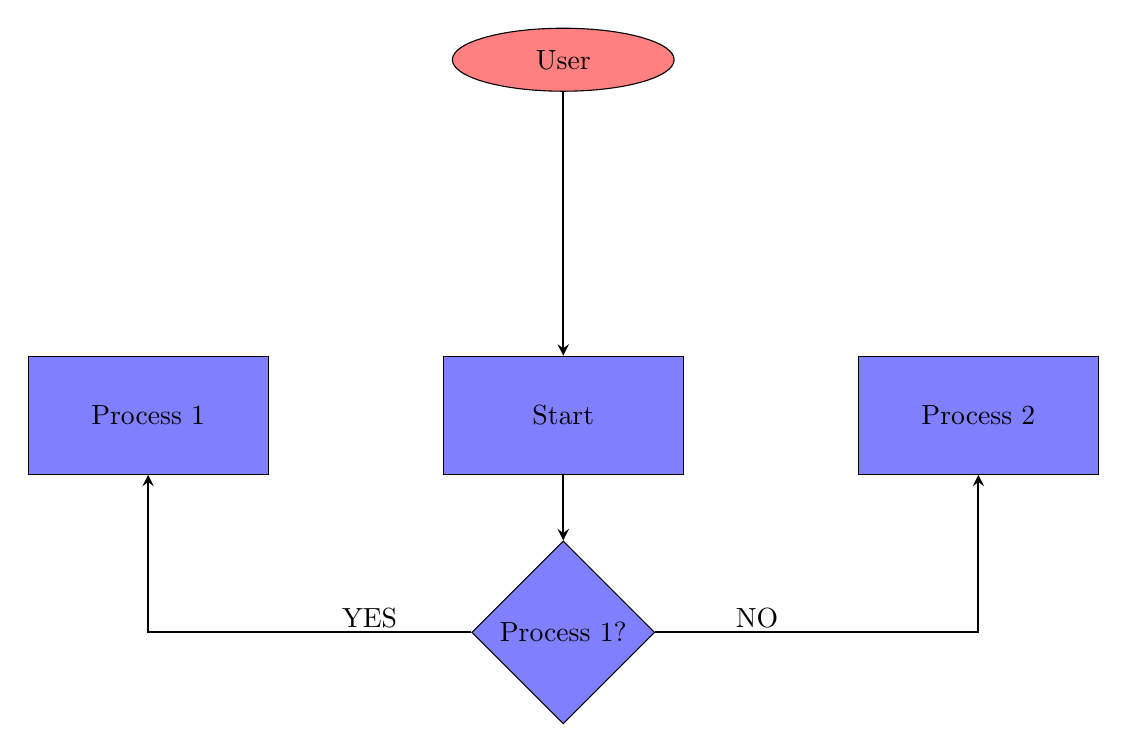
\begin{tikzpicture}

\tikzstyle{decision} = [diamond, draw, fill = blue!50]
\tikzstyle{line} = [draw, -stealth, thick]
\tikzstyle{elli} = [draw, ellipse, fill = red!50, minimum height = 8mm, 
	text width = 5em, text centered]
\tikzstyle{block} = [draw, rectangle, fill = blue!50, text width = 8em, 
	text centered, minimum height = 15mm, node distance = 10em]
\node [block](start){Start};
\node [block, left of  = start, xshift = -5em] (process 1){Process 1}; 
\node [elli, above of = start, yshift = 10em] (user) {User};
\node [block, right  of = start, xshift =5em] (process 2){Process 2};
\node [decision, below of = start, yshift = -5em](decision1) {Process 1?}; 
%arrows 
\path [line] (user) -- (start);
\path [line] (start) -- (decision1);
\path [line] (decision1) -| node [yshift = 0.5em, 
 	xshift = 8em] {YES} (process 1);
\path [line] (decision1) -| node [yshift = 0.5em, 
 	xshift = -8em] {NO} (process 2);

\end{tikzpicture}

\end{document}
